%%%%%%%%%%%%%%%%%%%%%%%%%%%%%%%%%%%%%%%%%%%%%%%%%%%%%%%%%%%%%%%%%%%%%%%%%%%%%%%%
%2345678901234567890123456789012345678901234567890123456789012345678901234567890
%        1         2         3         4         5         6         7         8

\documentclass[letterpaper, 10 pt, conference]{ieeeconf}  % Comment this line out if you need a4paper

%\documentclass[a4paper, 10pt, conference]{ieeeconf}      % Use this line for a4 paper

\IEEEoverridecommandlockouts                              % This command is only needed if 
                                                          % you want to use the \thanks command

\overrideIEEEmargins                                      % Needed to meet printer requirements.

%In case you encounter the following error:
%Error 1010 The PDF file may be corrupt (unable to open PDF file) OR
%Error 1000 An error occurred while parsing a contents stream. Unable to analyze the PDF file.
%This is a known problem with pdfLaTeX conversion filter. The file cannot be opened with acrobat reader
%Please use one of the alternatives below to circumvent this error by uncommenting one or the other
%\pdfobjcompresslevel=0
%\pdfminorversion=4

% See the \addtolength command later in the file to balance the column lengths
% on the last page of the document

% The following packages can be found on http:\\www.ctan.org
\usepackage{graphics} % for pdf, bitmapped graphics files
\usepackage{epsfig} % for postscript graphics files
\usepackage{mathptmx} % assumes new font selection scheme installed
\usepackage{times} % assumes new font selection scheme installed
\usepackage{amsmath} % assumes amsmath package installed
\usepackage{amssymb}  % assumes amsmath package installed
\usepackage[]{todonotes}
\usepackage{hyperref}
\usepackage[style=ieee]{biblatex}
\addbibresource{ref.bib}

\usepackage{booktabs}
\usepackage{multirow}
\usepackage{xcolor}
\usepackage{siunitx}
\sisetup{
  detect-all,
  exponent-product = \times,
  table-number-alignment = center,
}

% Real-time glyph in the headline table.  amssymb supplies \checkmark; guard it
% anyway so the generated table compiles under a minimal TeX installation.
\providecommand{\checkmark}{\ensuremath{\surd}}

% Explanatory note under a table.  IEEE typesets table captions in small caps,
% where a long caption becomes unreadable, so captions stay short titles and the
% detail lives here.  \linewidth is the float measure: \columnwidth in table,
% \textwidth in table*.
\newcommand{\tablenote}[1]{%
  \par\vspace{3pt}%
  \begin{minipage}{\linewidth}\footnotesize\raggedright #1\end{minipage}%
}

% The evaluation carries three full-width floats in one subsection, which the
% stock parameters cannot place: they defer past the bibliography.  Allowing
% more floats per page and a smaller text minimum keeps each float on or near
% the page that discusses it.
\renewcommand{\topfraction}{0.92}
\renewcommand{\bottomfraction}{0.7}
\renewcommand{\textfraction}{0.06}
\renewcommand{\floatpagefraction}{0.72}
\setcounter{topnumber}{3}
\setcounter{bottomnumber}{2}
\setcounter{totalnumber}{5}

\newcommand{\placeholder}{{\color{red}XX}}
\title{\LARGE \bf
Predictive Zonotope Reduction: Sound and Bounded-Memory Uncertainty Monitoring for Robotics
}


\author{Albert Author$^{1}$ and Bernard D. Researcher$^{2}$% <-this % stops a space
% \thanks{*This work was not supported by any organization}% <-this % stops a space
% \thanks{$^{1}$Albert Author is with Faculty of Electrical Engineering, Mathematics and Computer Science,
%         University of Twente, 7500 AE Enschede, The Netherlands
%         {\tt\small albert.author@papercept.net}}%
% \thanks{$^{2}$Bernard D. Researcheris with the Department of Electrical Engineering, Wright State University,
%         Dayton, OH 45435, USA
%         {\tt\small b.d.researcher@ieee.org}}%
}


\begin{document}



\maketitle
\thispagestyle{empty}
\pagestyle{empty}


%%%%%%%%%%%%%%%%%%%%%%%%%%%%%%%%%%%%%%%%%%%%%%%%%%%%%%%%%%%%%%%%%%%%%%%%%%%%%%%%
\begin{abstract}
\todo{LLM PLACEHOLDER ABSTRACT}
Set-based methods like zonotopes give sound, formally-grounded over-approximations of state under uncertainty, which makes them attractive for safety-critical robotics. Online, however, they do not scale: each step adds generators, and the usual fix — reducing the zonotope to a fixed order — either blows up memory or, when done offline, forces pessimistic worst-case input assumptions. Recent work achieves bounded-memory online reduction but commits to a single reduction method for the entire run. We observe that the reduction applied now affects the tightness of the set many steps later, so the choice of method is a sequential decision rather than a one-time configuration. We frame online zonotope reduction as a control problem — the action at each step is which reduction method to apply — and solve it with Model Predictive Control. The framing is sound by construction: every reduction is a sound over-approximation, so any schedule is too, and the choice affects only tightness, never safety. To meet real-time monitoring budgets, we distill the policy into a neural ranking policy with DAgger that matches, and in our experiments exceeds, online MPC while running far faster. Built on RTLola, a mature monitor with verified semantics and a ROS adapter, our method produces tighter reachable sets and fewer false-positive interventions than any single-method baseline, with bounded memory and real-time inference \todo{Make sure the tempalte didnt change}
\end{abstract}


\section{Introduction}
Robots acting in the physical world must make decisions under uncertainty. A mobile robot moving through clutter or a manipulator arm moving near a human does not observe a single exact state, but a set of states consistent with noisy sensors, model error, and actuation uncertainty.  Dealing with uncertainty requires methods computing possible reachable states, and if this set is too small, the robot may be allowed to performn an unsafe action. If it is too large, the safety monitor becomes overly conservative and triggers unnecessary stops or interventions. For safety-critical robotics, the central challenge is therefore not only to estimate uncertainty, but to track it soundly and tightly enough for online decisions. This also has impact on learning in robotics, as safety interruptions caused vacously slow down and break training in realistic robot settings.

Zonotopes are a natural representation for this problem  and are widely used from floating-point computation, neural network verification and computer grpahics, and have a rich use for reachability analysis in cyber-physical systems~\cite{Althoff2015ARCH,Wetzlinger2024diss}. They provide compact, sound over-approximations of reachable state sets and are closed under the linear operations needed for uncertainty propagation. 

However, their use in estimating uncertainty in cyber-physical systems suffers from a core trade-off between the performing these approximations online, and doing them offline.  Doing it offline, as in tools such as CORA~\cite{Althoff2015ARCH}, leads to \textit{pessimistic} overaproximations as it has to considers all  possible inputs which have to be presumed worst case, and not the actual ones that happen at runtime. On the other hand, approximating uncertainty with zonotopes online, with access to actually system inputs leads to a prohibitive memory blowup as every step adds generators, so the size of the zonotope representation grows without bound~\cite{DBLP:conf/rv/FinkbeinerFKK24}.


Recent work developing RLola~\cite{DBLP:journals/corr/cuttingcorners} shows you can combine both of these approaches through online reduction with bounded memory by compressing zonotopes on the fly during online computations. But just like CORA~\cite{Althoff2015ARCH} it commits to a single reduction method for the whole run. This misses a core insight: how you reduce the zonotope now, will impact how it will look in the future. Every reduction in zonotopes has impact both on the efficacy of reductions in the future, as well as what information is lost or preserved in the current step. Furthermore, the choice between all possible zonotope reduction methods is hard as there is a lot of them, and even more important: the best reduction is situation-dependent — different methods dominate in different regimes — so fixing one up front leaves tightness on the table, and worse, some methods quietly fail when their assumptions (e.g. invertibility) break.

In this paper, we show that we can improve uncertainty handling in montiroing by approaching zonotope reductions as a dynamic sequence problem. Unlike CORA~\cite{Althoff2015ARCH} or RLola~\cite{DBLP:journals/corr/cuttingcorners} approaches, which restricts the reduction method to be the same during the entire runtime of the system, we frame the problem as one of dynamic choice and allow different methods. To do it effectively, we frame this dynamic reductions as an optimal control problem, where the control action at each step is the seletion of the optimal zonotope reduction algorithm. We show that a dynamic ocntrol theory based approach outperform static zonotope reduction approaches.  Our framing is safe by construction: every individual reduction is a sound over-approximation, so any sequence of choices preserves the safety conditions required for safety-critical environemnts. 


To enable use in real-time systems we refine the method through several optimzation.  We reduce the computational overhead of MPC through search methods through the MPC policy via beam search, and push this even more by distilling the control policy into a neural one. We show that by distilling the control policy built through MPC into a neural one we get both a better policy, and one which runs significantly quicker then MPC and which actually can be deployed for real-time systems.

We build on Kohn et al by using RTLola monitor that provides us with strong formal guarantees. This gives us a strong foundation, as RTLola has seen extensive use in cyber-physical systems~\cite{DBLP:conf/cav/rtlolauav,DBLP:conf/cav/rtloltakeoff,DBLP:conf/tacas/BiewerFHKSS21,DBLP:conf/rv/ros}, and allows us to provide formal guarantees about the memory bounds, semantics and soundness of zonotope operations~\cite{DBLP:journals/sttt/rtlolaverguar,DBLP:conf/fm/semantics,DBLP:conf/rv/vermonitors}. We evaluate our method on the simulation of a 5-degrees-of-freedom robotic arm simulated in MuJoCo~\cite{todorov2012mujoco}, with the sensor noise and uncertainty being modelled according to ISO-5725~\cite{iso5725-1-2023}.

We show that our approach is outperforms others, both static zonotope reduction methods as seen in CORA and RLola. Our zonotopes are tighter, and the false positive rate is significantly lower. A lower FPR means that our method would cause less unnecessary emergency stops or task aborts - crucial both for safe operations in safety-critical environements as well as robot learning in uncertain environemnts where mistakes during exploration can cause damage or harm. Our method preserves soundness while reducing those false interventions.Furthermore, unlike probabilistic methods or Kalmans Filter based approaches our method provides concrete formal guarantees about hte over-approximations and makes it usable in safety critical environemnts. In comparison to offline methods, our method can take into account the actual inputs and give tigther expectations. This makes our work appropriate for safety-critical applications. 




We give the following contributions \todo{the contributions should be offline + online}
\begin{itemize} 
\item We formulate bounded-memory online zonotope reduction as an optimal control problem in which the monitor's action at each step is the choice of a sound reduction operator. This captures the central observation that reduction is not merely a local compression step: the reducer chosen at time $t$ changes the geometry of the zonotope available at later steps.
\item We instantiate this formulation with a receding-horizon MPC policy that selects reducers by optimizing predicted future set tightness. To meet real-time monitoring budgets, we distill the control policy into a DAgger-trained neural ranking policy that selects among sound reducers at runtime.
\item We implement predictive reducer selection in the RTLola monitoring framework with ROS integration and evaluate it on robotic systems under realistic measurement uncertainty. Compared with fixed-reducer baselines and offline/online variants, our method produces tighter reachable sets, reduces false-positive safety interventions, and achieves real-time inference while maintaining soundness and bounded memory. 
\end{itemize}

\section{Background}
\subsection{Zonotopes}
Math definition. Use in other domain
\subsection{Runtime Verification}
Runtime monitoring is an applied formal method that assures the safety of a running system by evaluating its behavior against a formal specification~\cite{DBLP:journals/jlp/LeuckerS09}. In particular, it has seen wide applications to cyber-physical systems, especially in safety-critical settings~\cite{DBLP:series/lncs/BartocciDDFMNS18, DBLP:conf/cav/rtlolauav,DBLP:conf/cav/rtloltakeoff,DBLP:journals/fmsd/MoosbruggerRS17}. A particularly powerful paradigm of runtime verification is the stream-based approach~\cite{DBLP:conf/time/DAngeloSSRFSMM05}, represented with tools such as TeSSLa~\cite{DBLP:conf/sbmf/TeSSla}, Striver~\cite{DBLP:conf/rv/Striver} or RTLola~\cite{DBLP:conf/cav/FaymonvilleFSSS19}. Here, the process runs through a specification  given in the form of terms of equations that relate input streams (that contain raw data such as sensor readings or actuator positions) to output streams (that transform and aggregate the incoming streams into information, or new streams themselves). The values on the output streams are then checked against trigger conditions that indicate faulty or dangerous situations and can be used to monitor or intervene into the operations of the system being observed. 
\paragraph{RTLola} In this paper, we primarly focus on RTLola, which has seen extensive used in autonomous and safety-critical systems including UAVs~\cite{DBLP:conf/cav/rtlolauav, DBLP:conf/cav/rtloltakeoff, dlr201362},  as well as deep integration into the robotics software stack via a ROS adapter~\cite{DBLP:conf/rv/ros}. The tool is validated in practice, supported on different hardware~\cite{DBLP:journals/tecs/fpga,BCFS25}, well documented~\cite{DBLP:conf/fm/rtlolatutorial,DBLP:conf/rv/rtloladesingandintegration}, and has an extensive formal methods foundations including memory bound guarantees, formally verified compilers and semantics~\cite{DBLP:journals/sttt/rtlolaverguar, DBLP:conf/rv/vermonitors,DBLP:conf/fm/semantics}. We provide a detailed definition of RTLola syntax and semantics in Appendix TODO.


\subsection{Model Predictive Control}
 \todo{TEMPORARY LLM PLACEHOLDER}
Model Predictive Control (MPC) is the standard receding-horizon approach to
optimal control. For a system $x_{k+1} = f(x_k, u_k)$, at each step $k$ the
controller observes the current state and solves a finite-horizon problem
%
\begin{equation}
  \min_{u_k,\dots,u_{k+H-1}}\ \sum_{j=0}^{H-1} \ell\big(x_{k+j}, u_{k+j}\big)
  \quad 
  \label{eq:mpc}
\end{equation}
%
where $H$ is the horizon and $\ell$ the stage cost. Only the first input
$u_k^\star$ is applied; the system advances, and the problem is re-solved from
the new state at $k+1$. Solving over a horizon requires a model of how the
system will evolve---in particular, a prediction of the future inputs over the
next $H$ steps.

In Section X we frame dynamic zonotope reduction as a MPC problem  with the action being the choice of reduction method and the stage
cost penalizing the size of the resulting set.

\subsection{Learning from Experts}
\label{sec:bg-imitation}
Imitation learning trains a policy to reproduce the decisions of an expert.  In our setting the expert is the control policy developed through Model Predictive Control reduction
policy and we distill it into a neural policy using DART?

\section{Related Work}
Conformal prediction for runtime monitoring + Symbolic pruning

MPC for uncertainty - Tube MPC etc.

Runtime Verification and uncertainty.  Lubeck people. Althoff people


\section{Uncertainty with Zonotopes}
Problem setting - why uncertainty is everywhere and why its important to be handled.  So you want to be safe, while still accounting for  Uncertainty you have some aproaches to measure in involve that uncertainty. This is also important for RL in robotics as learning in real-world environments needs to way to ensrue safety so you odnt crash the drone. Zonotopes for uncertainty in state as a way to do that.

Our definition of the uncertainty setup. We adapt the error model induced by the ISO5725~\cite{iso5725-1-2023} standard by decomposing the measurement error into a constant, but unknown per-sensor off-set and a randomly varying per-measurement error. This decomposition directly correlates with the “trueness” and “precision” described in the ISO 5725. 

% \todo{These paragrpah could arguably be removed? I covered most of hte points in the introduction already}
% \paragraph{Why not pick just one zonotope reduction method}

% Most work with online zonotopes leads to at least a linear memory blowup - which quickly become horrible in realistic settings. This is unpractical. Work of Kohn et al does the online zonotope reductions and has constant memory - but commits to one method of zonotope reduction. This approach misses the insigiht that reductions of the zonotope now actually matter for the future step. Futrthermore, while some methods are clearly better then other (as seen in Kohn et al, and also the CORA work) by mixing them we can be even better as different methods cover different subcases best

% \paragraph{Why not probabilistic Kalman Filter style methods}
% Kallman filters arent fail safe - concrete example of where they can fail. While sometimes you are okay with probabilistic methods, here we want compelte safety. Benefits of formal methods foundation, and that the reductions we have are sound


\subsection{Running Example}
A small toy example for intuition - omni robot. Small omni robot as in Kohn et al. Give dynamics, environment. Figure with a picture + RTLola spec. Motivate the story a bit and explain the spec and what RTLola does here with zonotopes.

The RTLOLA spec is indendent as it is supposed to monitor the system - its not that hard to specify behaviour, and the tool is already mature and supported with ROS etc.




\section{Predictive Zonotope Reductions}

Motivate the horizon and MPC as a good fit. Framing the Zonotope reduuctions as control decisions. 

Framing of the problem as a control problem. Definition of the state, action, step etc. as if this was control theory. 

We frame the online zonotope reduction as an online control problem. At each step we pick an action which is which method you pick. 

The cost function is evaluated against the unrolled zonotopes with approximation (can be done bounded in memory). We then evaluate the trajectories against that uncompressed one.

Importantly - we preserve soundness! As any choice you select is localy sound, so is the full trace.



\subsection{Offline Monitoring}
rollout mpc with the oracle, find optimal thing

In offline cases we have the full trace of inputs - we can do exact MPC optimisation over that. Recording the trace doesnt remove uncertainty!

More horizon = more performance but at exponential cost
More methods = more flexibility, but most of them suck. Shortly discuss all the CORA ones 

\subsection{Online Monitoring}
In the full online setting, we dont know the inputs in the future. We have two ways to handle this. One is to defer the horizon in a way, store the +H zonotopes fully, while predictiong the -H zonotope as if it was the offline setting.

In case that doesnt work, we can predict the inputs as well. As we dont see input, so we have to predict them so we interpolate. We tryed out some ismple methods and they basically work quite decently, so we do the stupid simple one.


The choice of interpolation barely matters.
On a horizon-3, width-4 beam we compared holding the last input against linear
and quadratic extrapolation: linear more than halves the forecast error
(normalized RMSE $0.464$ against hold, quadratic $0.488$), yet the three agree
to within \SI{2}{\percent} on every quantity the monitor cares about ---
false-positive rate \SIrange{0.565}{0.570}{\percent}, approximation loss
\numrange{1.28e-6}{1.43e-6}, and \SIrange{155.9}{158.9}{\milli\second} per event
--- with zero false negatives and zero executed fallbacks throughout.
A better forecast of the input does not buy a better reduction schedule, so we
keep the simplest predictor.
\todo{these numbers come from the superseded v2 run, not the v3 pipeline behind
Sec.~\ref{sec:evaluation}; rerun with input-predictor variation or drop}


doing the full rollout too expensive, so we do beam search. Show pareto vs fully known 



\subsection{Monitoring via Distillation}
While the MPC appraoch is better as we seen in Table X, it is also slow as it requires unrolling of the MPC and optimziation. Runtime verification has to run at lightspeed level shit.


To preserve the flexibility, and improving the speed of inference we distill the control policy. The neural net is tiny as we optimize for speed, and the inputs are matrix information (so not even the input is needed). We distill the control policy into this and show that it works really good and realyl quick.


Doing a classifier doesnt work, as it is really unbalanced dataset, and picking the minority actions when they matter is really important. thats why we dont learn a classifier, but a ranker. this is a much richer signal and handles the unbalance better


Table comparing the MPC selection vs Neural slection. Showing that it is almost the same (or even better) while being much faster - and still sound (as the reducers are sound) and memory bounded. 


\section{Evaluation}
\label{sec:evaluation}
We ask five questions.
Does treating reduction as a sequential decision produce tighter sets and fewer false interventions than any fixed reducer (Sec.~\ref{sec:eval-fixed})?
What does the predictive search cost, and how much of that cost is necessary (Sec.~\ref{sec:eval-search})?
Can that policy be made to run inside the monitor's real-time budget (Sec.~\ref{sec:eval-realtime})?
What does the symbolic guard change about the ensemble's decisions (Sec.~\ref{sec:eval-guard})?
And which reducers do the controllers actually select (Sec.~\ref{sec:eval-composition})?
Section~\ref{sec:eval-fixed-traces} closes with the controlled fault traces.
\todo[inline]{The prose in this section is deliberately thin: it states each
  result and leaves the detailed numbers to the floats. Write the full analysis
  after the final runs listed in \texttt{science/FINAL\_PAPER\_RUNS.md} land, and
  re-check every number quoted in the text against the regenerated artifacts.}

\subsection{Experimental Setup}
\label{sec:experimental-setup}
All experiments use the five-degree-of-freedom MuJoCo robot arm~\cite{todorov2012mujoco}, the packaged RTLola safety monitor, and the ISO~5725 measurement-error decomposition~\cite{iso5725-1-2023}.
We evaluate the seven binding transform bounds $b\in\{40,80,120,150,200,250,500\}$ against one exact unreduced reference per trace.

\paragraph{Metrics}
Our primary loss $\overline{L}$ is the event-mean binding-native approximation loss, and FPR uses exactly negative reference events as its denominator.
Because every reduction is individually sound, no method can produce a false negative by construction; accuracy differences are therefore differences in tightness and in the false interventions that looseness causes.
Throughput is event-loop throughput in events per second.
Traces advance at $\Delta t = \SI{0.1}{\second}$, so a monitor must sustain \SI{10}{\hertz} to keep pace with the system it observes; we treat that rate as the real-time budget throughout.
Relative throughput statements use paired cells, because concurrent execution affects absolute timing.
We also report \emph{availability}: the fraction of cells a method completes at all.
For a runtime monitor that is a first-class property, and one of the baselines does not have it.

\paragraph{Methods}
The canonical comparison covers the fixed Girard, Scott, PCA, and Combastel reducers; recorded-future terminal beam MPC (MPC-B); the one-event full-width teacher (MPC-F); causal predictive linear MPC (MPC-L); and three learned policies distilled from MPC-L.
G15/Clean148 is a single ranking policy trained on 148 clean teacher trajectories, Vote3 takes a plurality vote among three independently optimized \SI{5}{\percent}-DAgger specialists, and Vote3-Guarded adds a symbolic override to that vote.
MPC-B and MPC-F consume information a deployed monitor does not have and are accuracy references, not deployable policies.

\paragraph{Cohorts}
Generalization evidence comes from 20 held-out nominal random-waypoint traces (seeds 100--119) of 500 events each, giving 140 seed--budget cells per method.
The voting policies were evaluated on a second cohort of 20 previously untouched nominal seeds, 328--347, together with the teacher and the distilled policy, so the four learned rows in Sec.~\ref{sec:eval-realtime} are paired on identical traces.
The four full 2{,}340-event figure-eight traces --- nominal, drift, geofence, and drift plus geofence --- are controlled descriptive case studies and do not estimate a fault population.

\subsection{Dynamic Selection Against Fixed Reducers}
\label{sec:eval-fixed}
Table~\ref{tab:headline} and Fig.~\ref{fig:tradeoff} answer the first question, and the separation is not marginal.
Pooled over all 140 nominal cells, every fixed reducer produces a false positive on at least a third of negative events, while every dynamic selector stays at or below \SI{2.58}{\percent}, and the tightness gap between the best fixed reducer and MPC-L is roughly three and a half orders of magnitude.
Figure~\ref{fig:tradeoff}(a) places this in the plane that matters for deployment: the fixed reducers occupy the fast, loose region, the MPC variants occupy the tight, slow region and fall short of the \SI{10}{\hertz} rate at which the monitor stops keeping up with the system it watches, and the distilled policy is the only method in the lower-right quadrant.

\subsubsection*{A fixed schedule can fail outright}
The availability column records something the loss numbers cannot.
Scott completes 120 of its 140 nominal cells and \emph{none} of its 28 figure-eight cells: the run terminates once the looseness it has accumulated is large enough that its interval fallback can no longer be constructed.
Raising the bound delays that point by about ninety of the trace's 2{,}340 events rather than preventing it.
The failure is not a property of the trace.
On those same figure-eight traces Vote3-Guarded \emph{selects} Scott on the large majority of its over-bound decisions and meets zero infeasible candidates, and every MPC variant absorbs the identical failure at $b{=}40$ and still completes the cell.
A reducer that cannot be scheduled unconditionally is applied tens of thousands of times without incident when something else may be chosen in between.
That is the sequential coupling this paper is about, visible as a binary outcome rather than a ratio.

\begin{table}[t]
  \centering
  \caption{Held-out nominal generalization at $b=150$}
  \label{tab:headline}
  \small
  \setlength{\tabcolsep}{3.5pt}
  % Generated from the paired v4 final cohort; do not edit.
\begin{tabular}{l r S[table-format=2.2] c}
\toprule
Method & {$\overline{L}\downarrow$} & {FPR (\%)\,$\downarrow$} & {Cells} \\
\midrule
\multicolumn{4}{l}{\emph{Fixed reducer}} \\
\quad Girard & \num{6.7e-04} & 32.60 & 140/140 \\
\quad Scott & \num{7.6e+07} & 39.70 & \textbf{120}/140 \\
\quad PCA & \num{1.4e-01} & 62.11 & 140/140 \\
\quad Combastel & \num{6.4e-04} & 29.68 & 140/140 \\
\multicolumn{4}{l}{\emph{Offline oracle}} \\
\quad MPC-B & \num{1.5e-07} & 1.76 & 140/140 \\
\quad MPC-F & \num{2.1e-07} & 1.80 & 140/140 \\
\multicolumn{4}{l}{\emph{Online}} \\
\quad MPC-L & \bfseries \num{1.6e-07} & \bfseries 1.78 & 140/140 \\
\quad G15/Clean148 & \num{1.9e-07} & 5.08 & 140/140 \\
\quad Vote3 & \num{2.1e-07} & 1.92 & 140/140 \\
\quad Vote3-Guarded & \num{1.9e-07} & 1.79 & 140/140 \\
\bottomrule
\end{tabular}

  \tablenote{
    $\overline{L}$ and throughput are medians over 20 seeds; FPR is the
        macro mean with a paired-seed bootstrap. Bold marks the best value in
        each column among the causal methods; no method holds more than one.
        The offline oracles consume recorded future inputs or
        an exhaustive teacher and are accuracy references only. Real time is
        throughput $\geq\SI{10}{\hertz}$, the trace event rate. \emph{Cells}
        counts completed runs over the whole seven-bound sweep, not just the
        bound reported here. The two voting policies have been evaluated only on
        the confirmation cohort so far; their canonical rows are reserved and
        filled by the final run.
  }
\end{table}
\todo[inline]{Table~\ref{tab:headline} and Fig.~\ref{fig:tradeoff} reserve slots
  for Vote3 and Vote3-Guarded: both exist only on the confirmation cohort. One
  canonical run over seeds 100--119 fills them in, with no change to the
  generator.}
\begin{figure*}[t]
  \centering
  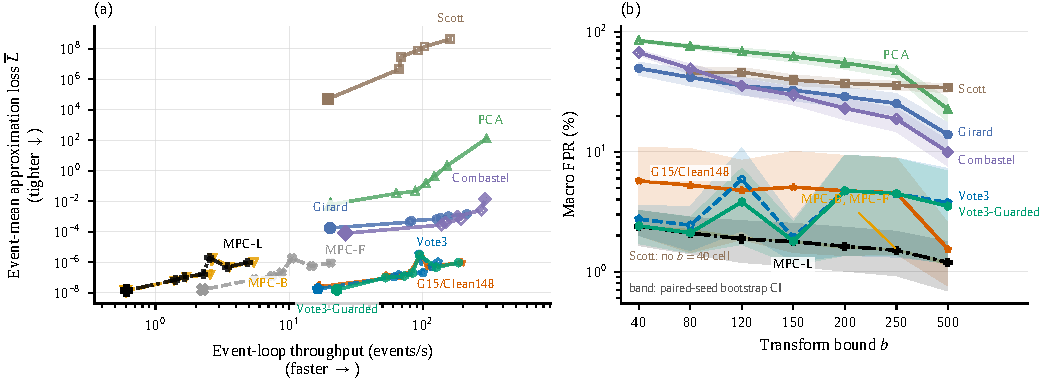
\includegraphics[width=\textwidth]{generated/accuracy_cost_tradeoff.pdf}
  \caption{
    Accuracy against cost on the held-out nominal seeds.
    (a) Each trail connects one method's seven transform bounds, from $b=40$ (open marker) to $b=500$ (filled marker); both axes are medians over 20 seeds.
    Every MPC variant stays under the \SI{10}{\hertz} trace event rate at every bound, which Table~\ref{tab:headline} records per method; the distilled policy attains MPC-scale loss above it.
    (b) Macro false-positive rate against the bound, the one axis the plane in (a) has no room for; the pale bands are paired-seed bootstrap \SI{95}{\percent} intervals, and the labelled envelope spans the two offline oracles, which is narrow enough to read as a line --- MPC-L stays within \SI{0.1}{pp} of it at every bound.
    Scott has no $b=40$ cell because its interval fallback fails there.
  }
  \label{fig:tradeoff}
\end{figure*}

\subsection{The Cost of Predictive Search}
\label{sec:eval-search}
Two design choices set the price of the MPC policy: how far the rollout looks ahead, and how wide the beam is.
Table~\ref{tab:search-cost} separates them on nominal seeds 60--64 at $b=150$, run single-worker so the timings are contention-free.

The horizon is worthless without a beam.
Every $W{=}1$ configuration returns exactly the same loss and the same FPR regardless of $H$: with one surviving candidate the rollout cannot change which reducer wins now, only how long it takes to confirm it.
Widening the beam to $W{=}2$ captures most of the available gain and further widening yields no consistent improvement, while the cost grows monotonically and steeply --- a factor of 26 in throughput across the grid.
Only the cheapest configurations meet the \SI{10}{\hertz} budget, and the configuration used elsewhere in this paper, $(4{,}4)$, is not among them.
This is the concrete reason distillation is necessary rather than merely convenient.
A matched cumulative stage objective, compared against the deployed terminal objective on the 28 paired fixed cells, is tighter on 16 of them; we read this as no meaningful separation at the scale that distinguishes dynamic from fixed selection, and retain the terminal objective because it is what the distillation teacher was defined against.

\begin{table}[t]
  \centering
  \caption{Cost of the predictive search: horizon and beam width}
  \label{tab:search-cost}
  \small
  {\setlength{\tabcolsep}{2.5pt}% Generated from frozen result artifacts; do not edit.
\begin{tabular}{l *{4}{r} c *{4}{S[table-format=2.1]}}
\toprule
 & \multicolumn{4}{c}{Median $\overline{L}$ ($\times 10^{-7}$)} & & \multicolumn{4}{c}{Median events/s} \\
\cmidrule(lr){2-5}\cmidrule(lr){7-10}
$H$ & {$W{=}1$} & {$W{=}2$} & {$W{=}4$} & {$W{=}8$} & & {$W{=}1$} & {$W{=}2$} & {$W{=}4$} & {$W{=}8$} \\
\midrule
1 & 2.91 & 1.67 & 1.59 & 1.59 & & \bfseries 45.9 & 31.8 & 20.6 & 20.5 \\
2 & 2.91 & \bfseries 1.27 & 1.40 & 1.51 & & 31.8 & 20.2 & 11.5 & 8.3 \\
4 & 2.91 & 1.48 & 1.61 & 1.68 & & 19.1 & 11.3 & 6.2 & 3.7 \\
8 & 2.91 & 1.70 & 1.28 & 1.63 & & 10.4 & 6.0 & 3.2 & 1.7 \\
\bottomrule
\end{tabular}
}
  \tablenote{
    Nominal seeds 60--64 at $b=150$, 80 cells, single worker so
        timings are contention-free; values are medians over five seeds. Bold
        marks the tightest and the fastest configuration in the grid, which are
        never the same one.
        $W{=}1$ is column-constant because a width-one beam admits no choice for
        the horizon to inform.
  }
\end{table}

\subsection{Three Learned Policies and the Real-Time Budget}
\label{sec:eval-realtime}
Distillation is what makes the teacher deployable, and the held-out cells support it on both axes.
The distilled ranking policy's median paired loss is within a factor of two of MPC-L, a policy that sees a full beam rollout, while MPC-L retains only \SI{2.62}{\percent} of its paired throughput.
The real-time claim is stronger than a median: across all 140 canonical nominal cells neither MPC-L nor MPC-B meets the \SI{10}{\hertz} budget in a single cell, whereas the distilled policy meets it in every one.

One policy is not the only way to distil a teacher, and the simplest one is also the most brittle.
Table~\ref{tab:learned} places three of them on the 140 untouched cells of seeds 328--347.
Plain distillation is tight in the centre but has the worst tail of the three.
Ensembling repairs the tail but pays for it in the centre, moving the median cell further from the teacher.
Adding the symbolic guard recovers the centre without giving the tail back: it is the tightest of the three at the median and at the ninetieth percentile, has the fewest severe cells, roughly halves the plain policy's macro false-positive rate, and sustains several times the monitoring budget.
Cell by cell it is tighter than plain distillation in 91 of 140 cells and than the unguarded vote in 115, and it retains the throughput of both.
We therefore take Vote3-Guarded as the learned policy of record.

One qualification belongs with that choice.
The severe tail is reduced, not eliminated: no learned policy reaches zero severe cells, and where the guard regresses it does so at the loosest bound.
This is consistent with a locally favourable override steering a later reduction adversely --- the same sequential coupling that motivates the method --- but the experiment does not isolate a causal mechanism.

\begin{table}[t]
  \centering
  \caption{Learned policies on the untouched confirmation cohort}
  \label{tab:learned}
  \footnotesize
  \setlength{\tabcolsep}{2.5pt}
  % Generated from the paired v4 final cohort; do not edit.
\begin{tabular}{l r S[table-format=1.2] r r S[table-format=2.0] S[table-format=1.2]}
\toprule
 & & \multicolumn{3}{c}{Loss ratio to MPC-L} & & \\
\cmidrule(lr){3-5}
Policy & {$\overline{L}$} & {p50} & {p90} & {p95} & {Sev.} & {FPR (\%)} \\
\midrule
MPC-L & \num{1.8e-07} & 1.00 & 1.00 & 1.00 & 0 & 1.78 \\
G15 & \bfseries \num{2.1e-07} & 1.28 & \num{2.49e+04} & \num{2.98e+08} & \bfseries 14 & 4.52 \\
Vote3 & \num{3.7e-07} & 1.39 & \num{6.09e+04} & \num{8.83e+07} & 19 & 3.71 \\
V3-Guard & \num{2.5e-07} & \bfseries 1.19 & \bfseries \num{2.74e+03} & \bfseries \num{6.41e+07} & \bfseries 14 & \bfseries 3.27 \\
\bottomrule
\end{tabular}

  \tablenote{
    140 cells, seeds 328--347, at seven transform bounds. $\overline{L}$ and
        throughput are medians; the quantile columns are per-cell paired ratios
        to the MPC-L teacher; Sev.\ counts cells beyond the preregistered
        $10^3$ severe threshold; FPR is the macro mean. Bold marks the best
        value among the three real-time policies; MPC-L is the accuracy
        reference and does not meet the \SI{10}{\hertz} budget.
        The median of the absolute losses and the median of the paired ratios
        need not agree, and here they do not: G15/Clean148 has the lower
        $\overline{L}$ while Vote3-Guarded wins cell for cell, because the two
        summarize different orderings of the same 140 cells.
        G15/Clean148 distils the teacher into one ranking policy, Vote3 votes
        among three DAgger specialists, and Vote3-Guarded adds the symbolic
        override to that vote.
  }
\end{table}

\subsection{What the Symbolic Guard Does}
\label{sec:eval-guard}
The override is deliberately small.
When the winning margin of the vote is at most one, it compares the current-event native loss of the reducers that received a vote and takes the best, breaking the deadlock with a measurement rather than a learned preference.
Figure~\ref{fig:guard} shows what that amounts to over the cohort's 69{,}120 over-bound decisions.
On \SI{94}{\percent} of them the three specialists agree outright and the guard cannot fire at all; it changes the outcome on \SI{2.8}{\percent} of all decisions, and amortizes to \SI{1.46}{\milli\second} per decision --- why the guarded policy is no slower than the unguarded one.

The flow itself is the interesting part, because it is not uniform.
The guard keeps Scott three times in four when the vote picks Scott, but overrides Girard three times in five, and the traffic runs almost entirely from Girard into Scott and Combastel.
The ensemble retains a residual preference for Girard that the measurement does not support, and the guard is mostly in the business of correcting it.
Section~\ref{sec:eval-composition} records the same shift from an independent source.

\begin{figure}[t]
  \centering
  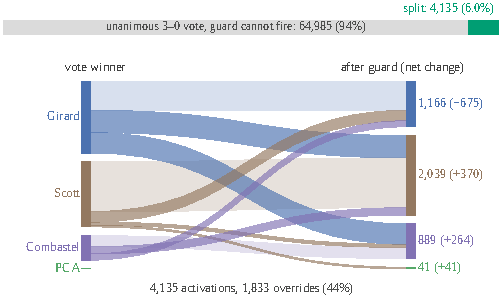
\includegraphics[width=\columnwidth]{generated/guard_flow.pdf}
  \caption{
    What the symbolic override changes, over the 69{,}120 over-bound decisions of the confirmation cohort.
    The bar gives the scale: on \SI{94}{\percent} of decisions the three specialists agree and the guard cannot engage.
    Below it, each band carries the decisions whose vote winner is on the left and whose executed reducer is on the right; pale bands are votes the guard leaves alone, saturated bands are overrides, and the bracketed figure is each reducer's net gain or loss.
    PCA is drawn as an empty lane: the three specialists cast one PCA vote between them in 69{,}120 decisions.
  }
  \label{fig:guard}
\end{figure}

\subsection{Reducer-Selection Preferences}
\label{sec:eval-composition}
Table~\ref{tab:reducer-composition} reports which ordinary reducers the controllers select.
All of them choose Scott on \SIrange{85}{89}{\percent} of valid reduction decisions, and the learned policies choose Girard on roughly \SIrange{9}{11}{\percent}.
Read against Table~\ref{tab:headline}, Scott's dominance is the paper's argument in one line: the reducer that is catastrophic --- and eventually fatal --- when applied unconditionally is the right choice most of the time, provided something else is available for the steps where it is not.
These are selection frequencies and not a causal decomposition; a reducer's utility depends on where it sits in the sequence.
Vote3-Guarded shifts \SI{1.6}{pp} from Girard to Combastel relative to the unguarded vote, the aggregate signature of the flow in Fig.~\ref{fig:guard} measured over a different set of decisions.

The learned policies also disagree with their teacher about one action.
Every MPC variant selects PCA on a small but non-zero fraction of decisions, and the distilled and voting policies have eliminated it almost entirely: \SI{0.14}{\percent} at most, and a single PCA vote in 69{,}120 over-bound decisions.
Distillation has pruned a minority action the teacher still uses.
That is defensible on these traces --- static PCA is the worst fixed reducer in Table~\ref{tab:headline} --- but it is the failure mode the ranking formulation was chosen to avoid, and we report it as an open weakness rather than a simplification.

\begin{table}[t]
  \centering
  \caption{Pooled reducer-selection frequencies (\%)}
  \label{tab:reducer-composition}
  \small
  % Generated from the paired v4 final cohort; do not edit.
\begin{tabular}{l *{4}{S[table-format=2.2]}}
\toprule
Controller & {Girard} & {Scott} & {PCA} & {Combastel} \\
\midrule
\quad MPC-B & 6.73 & \bfseries 85.55 & 3.03 & 4.69 \\
\quad MPC-F & 8.65 & \bfseries 84.24 & 2.38 & 4.73 \\
\quad MPC-L & 6.72 & \bfseries 85.56 & 3.20 & 4.52 \\
\quad G15/Clean148 & 10.99 & \bfseries 88.00 & 0.46 & 0.56 \\
\quad Vote3 & 10.41 & \bfseries 87.69 & 0.25 & 1.66 \\
\quad Vote3-Guarded & 9.13 & \bfseries 89.12 & 0.06 & 1.69 \\
\bottomrule
\end{tabular}

  \tablenote{
    Percentages condition on valid ordinary reduction decisions and
        exclude under-bound \texttt{none}, fallback, and infeasible decisions, so
        rows sum to 100; bold marks each controller's most-selected reducer.
        Each row aggregates 69{,}100--69{,}120 decisions. The two
        panels use distinct nominal seed cohorts and are interpreted within, not
        across, panels.
  }
\end{table}

\subsection{Controlled Figure-Eight Case Studies}
\label{sec:eval-fixed-traces}
Table~\ref{tab:figure8-summary} digests the four full-length figure-eight cases; the Appendix gives every cell.
These are single fixed traces, so they are a controlled record of behaviour under specific faults, not a population estimate; we read them for consistency with the nominal result rather than as independent evidence.
They are consistent.
The fixed reducers remain orders of magnitude looser at every bound, Scott completes nothing, and the four online policies stay within a factor of three of each other on every fault variant.
The dynamic policies hold FPR at or below \SI{1.1}{\percent} on every variant except two learned-policy excursions, which are the same over-triggering behaviour visible in Fig.~\ref{fig:tradeoff}(b).
On these traces the guard is unambiguously better than the vote it corrects: zero severe cells against three, and a lower worst-case loss ratio and pooled FPR.

\begin{table}[t]
  \centering
  \caption{Figure-eight fault variants, median over the seven bounds}
  \label{tab:figure8-summary}
  \footnotesize
  \setlength{\tabcolsep}{2.5pt}
  % Generated from frozen result artifacts; do not edit.
\begin{tabular}{l r r r r c}
\toprule
 & \multicolumn{4}{c}{Fault variant} & \\
\cmidrule(lr){2-5}
Method & {Nom.} & {Drift} & {Geo.} & {D+G} & {Cells} \\
\midrule
\multicolumn{6}{l}{\emph{Fixed}} \\
\quad Girard & \bfseries \num{8.9e-04} & \bfseries \num{7.2e-04} & \bfseries \num{9.8e-04} & \bfseries \num{8.2e-04} & 28/28 \\
\quad Scott & \num{4.7e+18}\rlap{$^{\dagger}$} & \num{4.2e+18}\rlap{$^{\dagger}$} & \num{4.7e+18}\rlap{$^{\dagger}$} & \num{4.2e+18}\rlap{$^{\dagger}$} & \textbf{0}/28 \\
\quad PCA & \num{1.9e+01} & \num{3.7e+00} & \num{2.8e+01} & \num{5.1e+00} & 28/28 \\
\quad Combastel & \num{1.6e-02} & \num{1.6e-02} & \num{1.7e-02} & \num{1.7e-02} & 28/28 \\
\multicolumn{6}{l}{\emph{Online}} \\
\quad MPC-L & \num{6.4e-07} & \num{6.3e-07} & \num{4.3e-07} & \num{4.2e-07} & 28/28 \\
\quad G15/Clean148 & \num{3.3e-07} & \num{2.8e-07} & \num{3.5e-07} & \num{3.0e-07} & 28/28 \\
\quad Vote3 & \bfseries \num{3.1e-07} & \num{4.2e-07} & \bfseries \num{3.0e-07} & \num{5.2e-07} & 28/28 \\
\quad Vote3-Guarded & \num{5.6e-07} & \bfseries \num{2.3e-07} & \num{6.1e-07} & \bfseries \num{2.4e-07} & 28/28 \\
\bottomrule
\end{tabular}

  \tablenote{
    Approximation loss $\overline{L}$, lower is better; median over the seven
        transform bounds. Bold marks the best value within each block of a
        column. The two offline oracles are omitted here and appear in
        Table~\ref{tab:headline} and Fig.~\ref{fig:tradeoff}.
        $^{\dagger}$Scott completes no cell; the value is the mean loss over the
        prefix before its interval fallback failed and is not comparable with a
        completed run; Sec.~\ref{sec:eval-fixed} reports where those runs end.
        The Appendix reports every bound and the
        corresponding false-positive rates.
  }
\end{table}

\section{Conclusion}
\section{Limitations}
The ML setup could be more interesting nad involved - especially direct zonotope data. We require the user to write a specification that monitors the system.
\todo{8 page limit}
\appendix[Complete Figure-Eight Results]
Tables~\ref{tab:figure8-loss} and~\ref{tab:figure8-fpr} give every cell behind
the digest in Table~\ref{tab:figure8-summary}: ten methods at seven transform
bounds on each of the four fault variants.

\begin{table*}[t]
  \centering
  \caption{Approximation loss $\overline{L}$ on the controlled figure-eight traces}
  \label{tab:figure8-loss}
  \footnotesize
  \setlength{\tabcolsep}{3pt}
  % Generated from frozen result artifacts; do not edit.
\begin{tabular}{l l r r r r r r r r r r}
\toprule
Trace & $b$ & \multicolumn{4}{c}{Fixed} & \multicolumn{2}{c}{Offline oracle} & \multicolumn{4}{c}{Online} \\
\cmidrule(lr){3-6}\cmidrule(lr){7-8}\cmidrule(lr){9-12}
 & & {Girard} & {Scott} & {PCA} & {Combast.} & {MPC-B} & {MPC-F} & {MPC-L} & {G15} & {Vote3} & {V3-Guard} \\
\midrule
Figure-8 & 40 & \bfseries \num{1.1e-03} & -- & \num{2.3e+02} & \num{4.3e-01} & \bfseries \num{4.7e-07} & \num{5.6e-07} & \num{5.9e-07} & \bfseries \num{5.6e-07} & \num{5.7e-07} & \bfseries \num{5.6e-07} \\
 & 80 & \bfseries \num{9.8e-04} & \num{1.4e+19}\rlap{$^{\dagger}$} & \num{2.2e+02} & \num{7.7e-02} & \num{7.1e-07} & \bfseries \num{3.5e-07} & \num{1.8e-06} & \num{3.3e-07} & \bfseries \num{3.1e-07} & \num{6.7e-07} \\
 & 120 & \bfseries \num{9.2e-04} & \num{6.0e+18}\rlap{$^{\dagger}$} & \num{6.5e+01} & \num{2.8e-02} & \bfseries \num{4.0e-06} & \num{4.6e-06} & \num{4.7e-06} & \num{4.1e-04} & \bfseries \num{3.3e-06} & \bfseries \num{3.3e-06} \\
 & 150 & \bfseries \num{8.9e-04} & \num{6.0e+18}\rlap{$^{\dagger}$} & \num{1.9e+01} & \num{1.6e-02} & \num{1.2e-06} & \bfseries \num{1.6e-07} & \num{1.1e-06} & \bfseries \num{1.5e-07} & \bfseries \num{1.5e-07} & \bfseries \num{1.5e-07} \\
 & 200 & \bfseries \num{8.2e-04} & \num{3.4e+18}\rlap{$^{\dagger}$} & \num{2.7e-01} & \num{9.1e-03} & \num{1.3e-07} & \bfseries \num{7.7e-08} & \num{6.4e-07} & \num{9.3e-08} & \num{9.3e-08} & \bfseries \num{9.1e-08} \\
 & 250 & \bfseries \num{7.7e-04} & \num{2.3e+18}\rlap{$^{\dagger}$} & \num{1.5e+01} & \num{5.4e-03} & \num{7.7e-07} & \bfseries \num{7.6e-08} & \num{2.9e-07} & \bfseries \num{5.4e-08} & \num{1.5e-07} & \num{6.8e-08} \\
 & 500 & \bfseries \num{6.0e-04} & \num{4.4e+17}\rlap{$^{\dagger}$} & \num{3.7e+00} & \num{1.3e-03} & \num{1.7e-08} & \bfseries \num{7.7e-09} & \bfseries \num{2.5e-08} & \num{3.1e-04} & \num{3.3e-05} & \num{8.0e-06} \\
\midrule
Figure-8 drift & 40 & \bfseries \num{9.1e-04} & -- & \num{4.8e+02} & \num{4.0e-01} & \num{3.6e-07} & \bfseries \num{3.1e-07} & \num{1.2e-06} & \bfseries \num{4.8e-07} & \num{4.9e-07} & \bfseries \num{4.8e-07} \\
 & 80 & \bfseries \num{8.2e-04} & \num{1.2e+19}\rlap{$^{\dagger}$} & \num{1.1e+02} & \num{6.7e-02} & \bfseries \num{2.5e-07} & \num{5.2e-07} & \num{8.1e-07} & \num{2.8e-07} & \num{4.2e-07} & \bfseries \num{2.3e-07} \\
 & 120 & \bfseries \num{7.6e-04} & \num{5.3e+18}\rlap{$^{\dagger}$} & \num{6.5e+00} & \num{2.5e-02} & \bfseries \num{3.6e-06} & \num{6.0e-06} & \num{4.1e-06} & \num{3.6e-04} & \bfseries \num{3.3e-06} & \bfseries \num{3.3e-06} \\
 & 150 & \bfseries \num{7.2e-04} & \num{5.8e+18}\rlap{$^{\dagger}$} & \num{3.7e+00} & \num{1.6e-02} & \num{1.8e-07} & \bfseries \num{1.2e-07} & \num{6.3e-07} & \bfseries \num{1.2e-07} & \num{1.3e-07} & \bfseries \num{1.2e-07} \\
 & 200 & \bfseries \num{6.9e-04} & \num{3.1e+18}\rlap{$^{\dagger}$} & \num{3.4e+00} & \num{8.4e-03} & \num{2.3e-07} & \bfseries \num{6.3e-08} & \num{1.2e-07} & \num{7.8e-08} & \num{7.8e-08} & \bfseries \num{7.5e-08} \\
 & 250 & \bfseries \num{6.3e-04} & \num{2.1e+18}\rlap{$^{\dagger}$} & \num{4.5e-01} & \num{5.5e-03} & \bfseries \num{5.1e-08} & \num{2.0e-07} & \num{5.6e-07} & \bfseries \num{4.5e-08} & \num{7.0e-08} & \num{4.6e-08} \\
 & 500 & \bfseries \num{5.1e-04} & \num{3.5e+17}\rlap{$^{\dagger}$} & \num{2.5e+00} & \num{1.3e-03} & \num{3.6e-08} & \bfseries \num{1.1e-08} & \bfseries \num{2.5e-08} & \num{3.2e-04} & \num{1.1e-04} & \num{5.6e-06} \\
\midrule
Figure-8 geofence & 40 & \bfseries \num{1.2e-03} & -- & \num{7.1e+02} & \num{4.3e-01} & \bfseries \num{7.2e-07} & \num{1.0e-06} & \num{7.0e-07} & \bfseries \num{6.1e-07} & \num{6.2e-07} & \bfseries \num{6.1e-07} \\
 & 80 & \bfseries \num{1.1e-03} & \num{1.4e+19}\rlap{$^{\dagger}$} & \num{4.9e+02} & \num{7.4e-02} & \bfseries \num{5.2e-07} & \num{6.6e-07} & \num{5.4e-07} & \num{3.5e-07} & \bfseries \num{3.0e-07} & \num{6.9e-07} \\
 & 120 & \bfseries \num{1.0e-03} & \num{6.0e+18}\rlap{$^{\dagger}$} & \num{4.1e+02} & \num{2.7e-02} & \num{5.2e-06} & \bfseries \num{4.9e-06} & \num{3.9e-06} & \num{5.3e-04} & \bfseries \num{3.3e-06} & \bfseries \num{3.3e-06} \\
 & 150 & \bfseries \num{9.8e-04} & \num{6.0e+18}\rlap{$^{\dagger}$} & \num{2.2e+01} & \num{1.7e-02} & \num{8.4e-07} & \bfseries \num{2.9e-07} & \num{4.3e-07} & \bfseries \num{1.6e-07} & \bfseries \num{1.6e-07} & \bfseries \num{1.6e-07} \\
 & 200 & \bfseries \num{9.2e-04} & \num{3.4e+18}\rlap{$^{\dagger}$} & \num{1.9e-01} & \num{9.3e-03} & \num{2.5e-07} & \bfseries \num{8.2e-08} & \num{3.7e-07} & \num{9.8e-08} & \num{9.8e-08} & \bfseries \num{9.4e-08} \\
 & 250 & \bfseries \num{8.6e-04} & \num{2.3e+18}\rlap{$^{\dagger}$} & \num{2.8e+01} & \num{5.6e-03} & \num{6.7e-07} & \bfseries \num{8.2e-08} & \num{2.6e-07} & \bfseries \num{5.6e-08} & \num{5.7e-08} & \bfseries \num{5.6e-08} \\
 & 500 & \bfseries \num{6.7e-04} & \num{4.4e+17}\rlap{$^{\dagger}$} & \num{6.0e+00} & \num{1.4e-03} & \num{1.8e-08} & \bfseries \num{9.6e-09} & \bfseries \num{3.7e-08} & \num{3.4e-04} & \num{3.0e-05} & \num{6.4e-06} \\
\midrule
Figure-8 drift + geofence & 40 & \bfseries \num{1.0e-03} & -- & \num{4.6e+02} & \num{4.4e-01} & \num{5.1e-07} & \num{5.1e-07} & \num{9.8e-07} & \bfseries \num{5.3e-07} & \num{5.4e-07} & \bfseries \num{5.3e-07} \\
 & 80 & \bfseries \num{9.2e-04} & \num{1.2e+19}\rlap{$^{\dagger}$} & \num{1.3e+02} & \num{7.4e-02} & \bfseries \num{3.4e-07} & \num{1.5e-06} & \num{4.2e-07} & \num{3.0e-07} & \num{5.2e-07} & \bfseries \num{2.4e-07} \\
 & 120 & \bfseries \num{8.7e-04} & \num{5.3e+18}\rlap{$^{\dagger}$} & \num{6.8e+00} & \num{2.8e-02} & \bfseries \num{4.9e-06} & \num{6.0e-06} & \num{5.5e-06} & \num{4.7e-04} & \bfseries \num{3.3e-06} & \bfseries \num{3.3e-06} \\
 & 150 & \bfseries \num{8.2e-04} & \num{5.8e+18}\rlap{$^{\dagger}$} & \num{5.1e+00} & \num{1.7e-02} & \num{7.9e-07} & \bfseries \num{2.5e-07} & \num{8.9e-07} & \bfseries \num{1.3e-07} & \num{1.4e-07} & \bfseries \num{1.3e-07} \\
 & 200 & \bfseries \num{7.6e-04} & \num{3.1e+18}\rlap{$^{\dagger}$} & \num{3.2e+00} & \num{8.9e-03} & \bfseries \num{2.3e-07} & \num{2.9e-07} & \num{1.3e-07} & \num{8.2e-08} & \num{8.2e-08} & \bfseries \num{7.9e-08} \\
 & 250 & \bfseries \num{7.2e-04} & \num{2.1e+18}\rlap{$^{\dagger}$} & \num{2.8e+00} & \num{5.5e-03} & \bfseries \num{4.8e-08} & \num{2.0e-07} & \num{2.6e-07} & \bfseries \num{4.7e-08} & \num{5.0e-08} & \bfseries \num{4.7e-08} \\
 & 500 & \bfseries \num{5.6e-04} & \num{3.5e+17}\rlap{$^{\dagger}$} & \num{2.2e+00} & \num{1.3e-03} & \num{4.8e-08} & \bfseries \num{1.7e-08} & \bfseries \num{4.8e-08} & \num{3.5e-04} & \num{7.8e-05} & \num{7.6e-06} \\
\bottomrule
\end{tabular}

  \tablenote{
    Lower is better; bold marks the best value within each column block of a
        row, and a block whose entries all tie is left unmarked. MPC-B and MPC-F
        consume recorded future inputs or an exhaustive teacher and are accuracy
        references rather than deployable policies, so they are ranked among
        themselves rather than against the causal policies.
        $^{\dagger}$Scott completes no cell in this table; the value is the mean
        loss over the prefix before its interval fallback failed, is not
        comparable with a completed run, and never takes the best-in-block mark.
        Sec.~\ref{sec:eval-fixed} reports where each of those runs ends.
  }
\end{table*}

\begin{table*}[t]
  \centering
  \caption{False-positive rate (\%) on the controlled figure-eight traces}
  \label{tab:figure8-fpr}
  \small
  \setlength{\tabcolsep}{4pt}
  % Generated from frozen result artifacts; do not edit.
\begin{tabular}{l l S[table-format=2.2] S[table-format=2.2] S[table-format=2.2] S[table-format=2.2] S[table-format=2.2] S[table-format=2.2] S[table-format=2.2] S[table-format=2.2] S[table-format=2.2] S[table-format=2.2]}
\toprule
Trace & $b$ & \multicolumn{4}{c}{Fixed} & \multicolumn{2}{c}{Offline oracle} & \multicolumn{4}{c}{Online} \\
\cmidrule(lr){3-6}\cmidrule(lr){7-8}\cmidrule(lr){9-12}
 & & {Girard} & {Scott} & {PCA} & {Combast.} & {MPC-B} & {MPC-F} & {MPC-L} & {G15} & {Vote3} & {V3-Guard} \\
\midrule
Figure-8 & 40 & \bfseries 51.67 & {--} & 97.48 & 94.27 & 0.00 & 0.00 & 0.00 & 0.00 & 0.00 & 0.00 \\
 & 80 & \bfseries 41.79 & {--} & 95.90 & 90.51 & 0.00 & 0.00 & 0.00 & 0.00 & 0.00 & 0.00 \\
 & 120 & \bfseries 33.46 & {--} & 93.80 & 86.75 & 0.00 & 0.00 & \bfseries 0.00 & 10.30 & \bfseries 0.00 & \bfseries 0.00 \\
 & 150 & \bfseries 26.88 & {--} & 93.72 & 83.08 & 0.00 & 0.00 & 0.00 & 0.00 & 0.00 & 0.00 \\
 & 200 & \bfseries 23.46 & {--} & 76.97 & 77.14 & 0.00 & 0.00 & 0.00 & 0.00 & 0.00 & 0.00 \\
 & 250 & \bfseries 16.37 & {--} & 91.37 & 73.33 & 0.00 & 0.00 & 0.00 & 0.00 & 0.00 & 0.00 \\
 & 500 & \bfseries 2.22 & {--} & 83.42 & 44.96 & 0.00 & 0.00 & \bfseries 0.00 & 7.39 & \bfseries 0.00 & \bfseries 0.00 \\
\midrule
Figure-8 drift & 40 & \bfseries 12.32 & {--} & 97.05 & 92.94 & 0.00 & 0.00 & 0.00 & 0.00 & 0.00 & 0.00 \\
 & 80 & \bfseries 5.32 & {--} & 95.37 & 88.36 & 0.00 & 0.00 & 0.00 & 0.00 & 0.00 & 0.00 \\
 & 120 & \bfseries 1.37 & {--} & 93.10 & 83.04 & 0.00 & 0.00 & \bfseries 0.00 & 0.63 & \bfseries 0.00 & \bfseries 0.00 \\
 & 150 & \bfseries 1.79 & {--} & 91.36 & 79.99 & 0.00 & 0.00 & 0.00 & 0.00 & 0.00 & 0.00 \\
 & 200 & \bfseries 0.00 & {--} & 89.31 & 72.78 & 0.00 & 0.00 & 0.00 & 0.00 & 0.00 & 0.00 \\
 & 250 & \bfseries 0.00 & {--} & 76.51 & 65.98 & 0.00 & 0.00 & 0.00 & 0.00 & 0.00 & 0.00 \\
 & 500 & \bfseries 0.00 & {--} & 76.09 & 29.91 & 0.00 & 0.00 & 0.00 & 0.00 & 0.00 & 0.00 \\
\midrule
Figure-8 geofence & 40 & \bfseries 57.96 & {--} & 96.52 & 92.10 & \bfseries 0.71 & 0.88 & 0.83 & \bfseries 0.65 & \bfseries 0.65 & \bfseries 0.65 \\
 & 80 & \bfseries 45.34 & {--} & 94.34 & 86.91 & 0.71 & 0.71 & \bfseries 0.24 & 0.41 & 0.35 & 0.47 \\
 & 120 & \bfseries 37.32 & {--} & 91.45 & 81.72 & \bfseries 0.24 & 0.47 & 0.47 & 18.40 & 0.35 & \bfseries 0.29 \\
 & 150 & \bfseries 32.96 & {--} & 91.33 & 76.65 & 0.47 & \bfseries 0.24 & 0.35 & 0.29 & 0.29 & \bfseries 0.24 \\
 & 200 & \bfseries 28.07 & {--} & 67.39 & 68.46 & 0.18 & 0.18 & \bfseries 0.12 & 0.41 & 0.41 & 0.35 \\
 & 250 & \bfseries 24.47 & {--} & 88.09 & 63.21 & \bfseries 0.12 & 0.24 & \bfseries 0.06 & 0.18 & 0.12 & 0.18 \\
 & 500 & \bfseries 21.23 & {--} & 77.12 & 24.59 & 0.12 & 0.12 & \bfseries 0.12 & 13.74 & 5.48 & 1.83 \\
\midrule
Figure-8 drift + geofence & 40 & \bfseries 25.73 & {--} & 96.64 & 91.96 & \bfseries 0.84 & 0.90 & \bfseries 0.84 & 1.02 & 1.02 & 1.02 \\
 & 80 & \bfseries 21.18 & {--} & 94.72 & 86.74 & 0.84 & \bfseries 0.42 & 0.84 & \bfseries 0.72 & 0.84 & \bfseries 0.72 \\
 & 120 & \bfseries 20.52 & {--} & 92.14 & 80.68 & 0.84 & 0.84 & \bfseries 0.48 & 16.20 & \bfseries 0.48 & 0.66 \\
 & 150 & \bfseries 20.52 & {--} & 90.16 & 77.20 & 0.66 & \bfseries 0.60 & 0.60 & \bfseries 0.36 & 0.42 & \bfseries 0.36 \\
 & 200 & \bfseries 20.16 & {--} & 87.82 & 68.99 & 0.78 & \bfseries 0.60 & 0.66 & \bfseries 0.42 & \bfseries 0.42 & \bfseries 0.42 \\
 & 250 & \bfseries 19.38 & {--} & 73.25 & 61.25 & 0.48 & \bfseries 0.36 & 0.48 & 0.36 & \bfseries 0.30 & 0.42 \\
 & 500 & \bfseries 18.36 & {--} & 72.77 & 24.36 & \bfseries 0.36 & 0.48 & 0.48 & 11.28 & 6.78 & \bfseries 0.42 \\
\bottomrule
\end{tabular}

  \tablenote{
    Lower is better; columns and the bold convention match
        Table~\ref{tab:figure8-loss}. Scott has no entry because it completes no
        cell. Most rows leave the online block unmarked
        because all four policies reach \SI{0.00}{\percent} there; bold appears
        only where they separate.
  }
\end{table*}

\printbibliography




\end{document}
